\documentclass[11pt]{article}
\usepackage{mypackages}
\begin{document}

\maketitle

\section{Actor Critic}

In reinforcement learning there there are two paradigms for how the learning progress evaluating, the paradigms are called value-iteration and policy-iteration. In Q-learning you are using value-iteration and in SARSA you are using policy-iteration. What is diffrence between these?

\subsection{Value iteration}

Reinforcement learning algorithms which using Value iteration for learning, try to estimates a value function $V(s)$, which describe how good a certain state $s$ is to be in. Given a discrete state space, you can imagine that every state has is own estimated value, which tells the expected reward for be given in that state. The algorithms often using a greedy policy for taking a action $a$ which maximize the value function. 

\subsection{Policy iteration}


Reinforcement learning algorithm using Policy iteration for learning, try to estimate the optimal policy for a given state $\pi(s)$ (a set of action probabilities). Given a discrete state space, you can imagine that every state, have a set of the probabilities, where every element in the set is a probability for that action will maximize the reward. When a policy iteration algorithm converges, we see that one action given state $s$ will get a high probability, but as long the others actions still have a probability higher than 0, they will still be executed some times, which help the algorithm to not be stock in local minimum.

\subsection{Actor Critic}



At figure (REFERNCE TIL FIGUR OMKRING REIFORCEMENT LEARNING) we saw a illustration of how reinforcment learning works. In actor critic we combine the benefits from both Value iteration and Policy iteration. Here we see a illustration of how an actor critic model is structured


\begin{figure}[H]
    \centering
    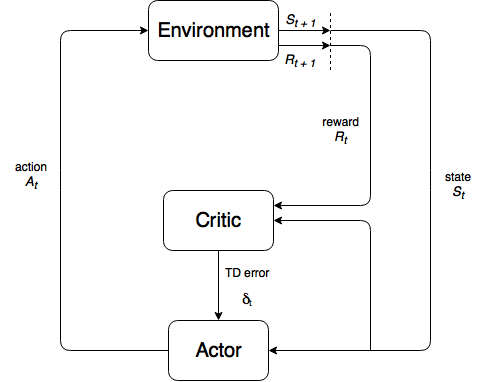
\includegraphics[scale=0.5]{include/ActorCriticDiagram.png}
    \caption{A model of the actor critic structure}
    \label{fig:actor_critic}
\end{figure}




%\printbibliography
%\bibliography{citations}
%\bibliographystyle{plain}
\end{document}
